\chapter{Approximate Dynamic Programming}
\label{chapter: ADP}

%%\parbox[pos][height][contentpos]{width}{text}



%%\begin{minipage}[pos][height][contentpos]{width} text \end{minipage}

\begin{minipage}{5in} 
ทดสอบ minipage
\end{minipage}

\fbox{
\begin{minipage}{\textwidth} 
ทดสอบ minipage
It is natural but wrong to visualize the singularity as a kind of pregnant dot hanging in a dark, boundless void. But there is no space, no darkness. The singularity has no “around” around it. There is no space for it to occupy, no place for it to be. We can’t even ask how long it has been there—whether it has just lately popped into being, like a good idea, or whether it has been there forever, quietly awaiting the right moment. Time doesn’t exist. There is no past for it to emerge from.
And so, from nothing, our universe begins.
\end{minipage}
}


%
\begin{figure}
\begin{center}
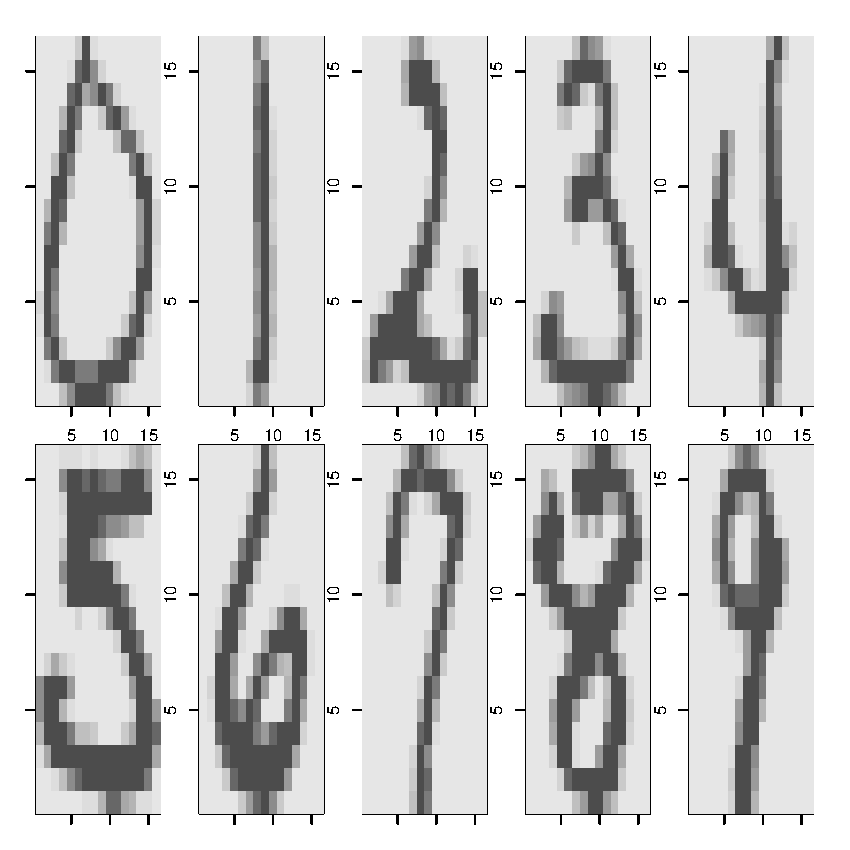
\includegraphics[width=2.0in]
{01Intro/zipdigits.eps}
\end{center}
\caption{ตัวอย่างรูปทดสอบใน shaded}
%%\label{fig: example ZIP image digits}
\end{figure}
%

\begin{shaded}
ทดสอบ shaded
I’m assuming of course that you wish to build an inflationary universe. If you’d prefer instead to build a more old-fashioned, standard Big Bang universe, you’ll need additional materials. In fact, you will need to gather up everything there is every last mote and particle of matter between here and the edge of creation and squeeze it into a spot so infinitesimally compact that it has no dimensions at all. It is known as a singularity.
In either case, get ready for a really big bang. Naturally, you will wish to retire to a safe place to observe the spectacle. Unfortunately, there is nowhere to retire to because outside the singularity there is no where. When the universe begins to expand, it won’t be spreading out to fill a larger emptiness. The only space that exists is the space it creates as it goes.
\end{shaded}

%\begin{snugshaded}
%ทดสอบ shaded
%\end{snugshaded}

\begin{mdframed}[backgroundcolor=yellow]
ทดสอบ mdframed
เกร็ดเล็กเกร็ดน้อย
NO MATTER HOW hard you try you will never be able to grasp just how tiny, how spatially unassuming, is a proton. It is just way too small.
A proton is an infinitesimal part of an atom, which is itself of course an insubstantial thing. Protons are so small that a little dib of ink like the dot on this i can hold something in the region of 500,000,000,000 of them, rather more than the number of seconds contained in half a million years. So protons are exceedingly microscopic, to say the very least.
Now imagine if you can (and of course you can’t) shrinking one of those protons down to a billionth of its normal size into a space so small that it would make a proton look enormous. Now pack into that tiny, tiny space about an ounce of matter. Excellent. You are ready to start a universe.
\end{mdframed}

\begin{displaymath}
    \xymatrix{
        A \ar[d] \ar[dr] \ar[drr] &   &   \\
        B                         & C & D }
\end{displaymath}

\section{Quotes}

``Finally, we want to emphasize that reinforcement learning is meant to be a \textit{general} approach to learning from interaction. It is general enough not to require special purpose teachers and domain knowledge, but also general enough to utilize such things if they are available.'' Sutton \& Barto 1998 (pp. 260)

\section{Akaike Information Criteria for K-means}

%\begin{verse}
`` dummy quote '', dummy author
%\end{verse}

เราคำนวณค่าเอไอซีได้จากสมการ~\ref{eq: AIC for K-means}.
แนวคิดของเอไอซี คือ เราจะเลือกโมเดลที่ให้ค่าเอไอซีน้อยที่สุด $M = \arg\min_{\kappa} \mathrm{AIC}(\kappa)$.

\begin{eqnarray}
   \mathrm{AIC}(\kappa) &=& -2 \cdot \log L + 2 \cdot M_{\theta} 
\nonumber \\
   &=& \mathrm{RSS}^*(\kappa) + 2 \cdot \kappa \cdot D 
\label{eq: AIC for K-means} \\
   \mathrm{RSS}^*(\kappa) &=& \min_{\pi \in \Pi(\kappa)} \mathrm{RSS}^{\pi} (\kappa)
\label{eq: best clustering RSS} \\
\mathrm{RSS}^{\pi} (\kappa) &=& \sum_{m=1}^{\kappa} \mathrm{RSS}^{\pi}_m
\label{eq: clustering RSS} \\
\mathrm{RSS}^{\pi}_m &=& \sum_{\vec{x} \in \Omega_m^{\pi}} \| \vec{x} - \vec{\mu}_m^{\pi} \|^2
\label{eq: cluster RSS}
\end{eqnarray}


\subsection{Nonparametric Methods}

%
\begin{figure}
\begin{center}
\includegraphics[width=5.5in]{08KNN/replicateFig2_24.eps}
\end{center}
\caption{การใช้ฮิสโตแกรมประมาณการแจกแจง}
\label{fig: ch03 nonparam histogram}
\end{figure}

